
\subsection{Datasets}
\begin{table}
\resizebox{1\columnwidth}{!}{
\begin{tabular}{ll|cc|c}
Language&&Size (MB)&Tokens (M)& Sentences (K)\\
\toprule 
Bulgarian&BG&36.11&8.53&329\\
Czech&CS&53.48&12.25&535\\
German&DE&171.80&44.07&1785 \\
English&EN&179.15&49.32&1815\\
Finnish&FI&145.32&32.85&1737\\
French&FR&197.68&53.82&1792\\
Hungarian&HU&52.53&12.02&527\\
Italian&IT&186.67&48.08&1703\\
Portuguese&PT&187.20&49.03&1737\\
\end{tabular}}
\caption{Data statistics after tokenizing, sentence-splitting, and removing markups, and numberizing. Tokens and sentence counts refer to the training partition. \trevor{Move to \supp}}
\end{table}

\begin{figure}
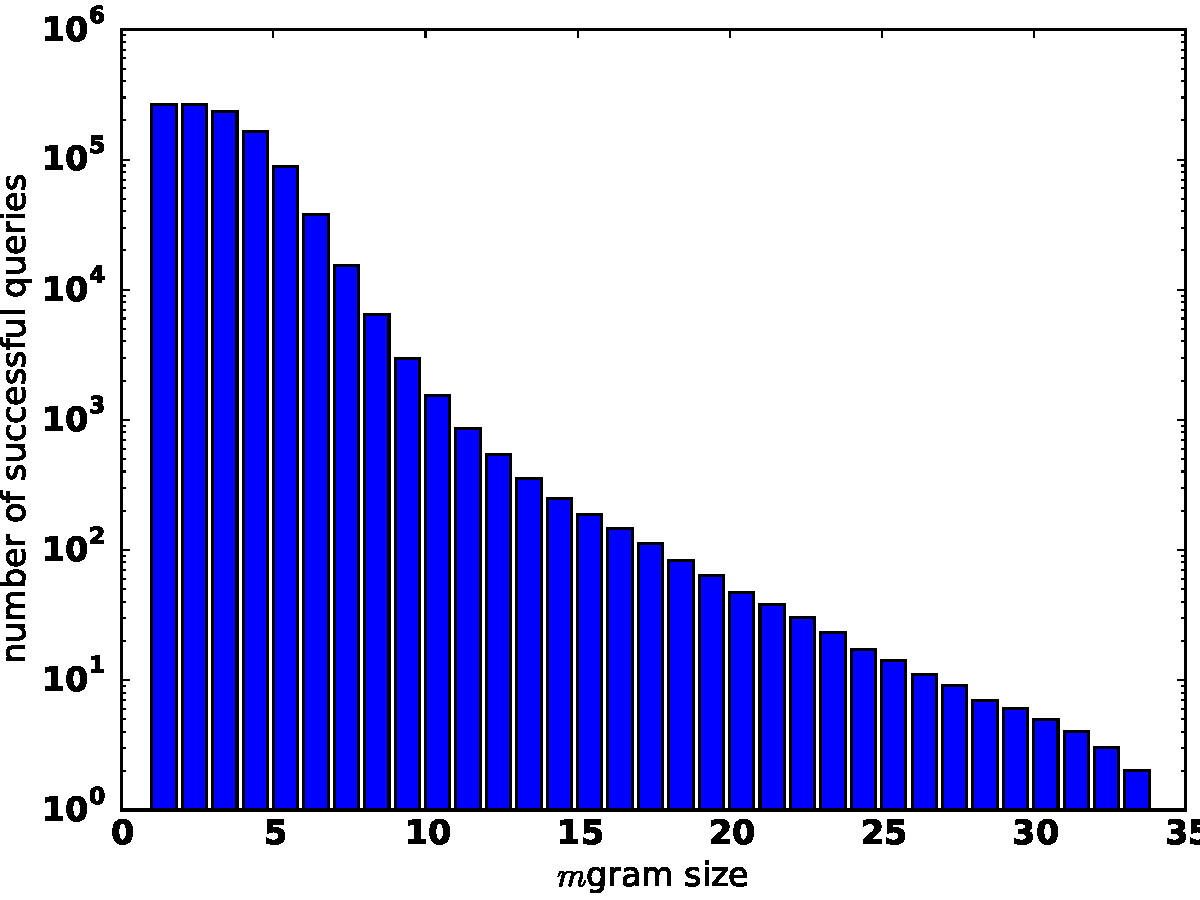
\includegraphics[width=\columnwidth]{figures/german_pattern_size.pdf}
\caption{Number of successful queries across different pattern sizes from KN computation over the German test set, with unbounded $m$.}
\end{figure}

\begin{figure}
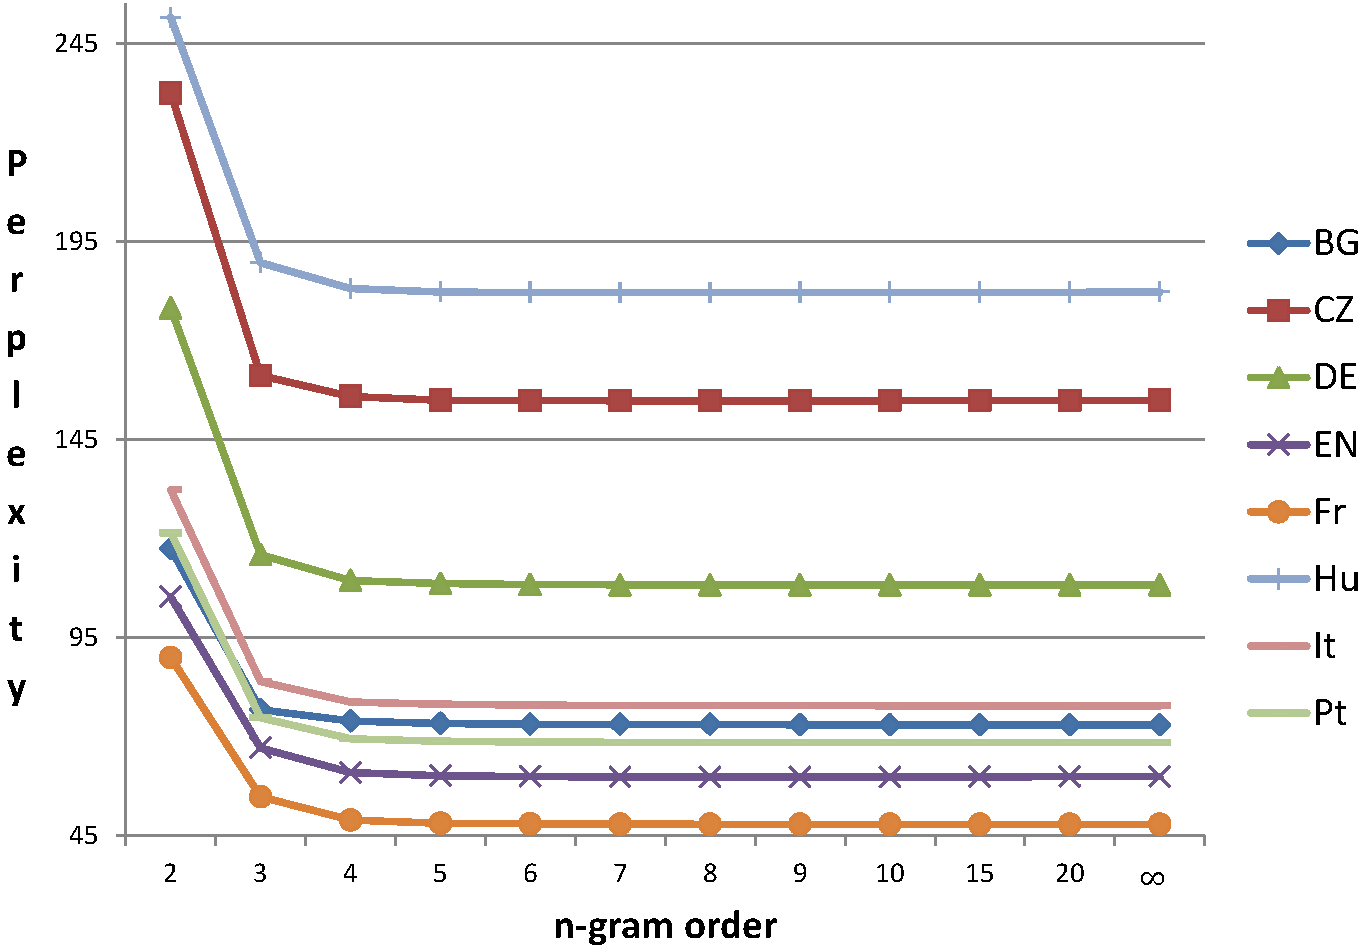
\includegraphics[width=\columnwidth]{figures/Perplexity-n.pdf}
\caption{All 8 languages pplx results with m=2..10,15,20,infinity(=99999).}
\end{figure}

\begin{figure}
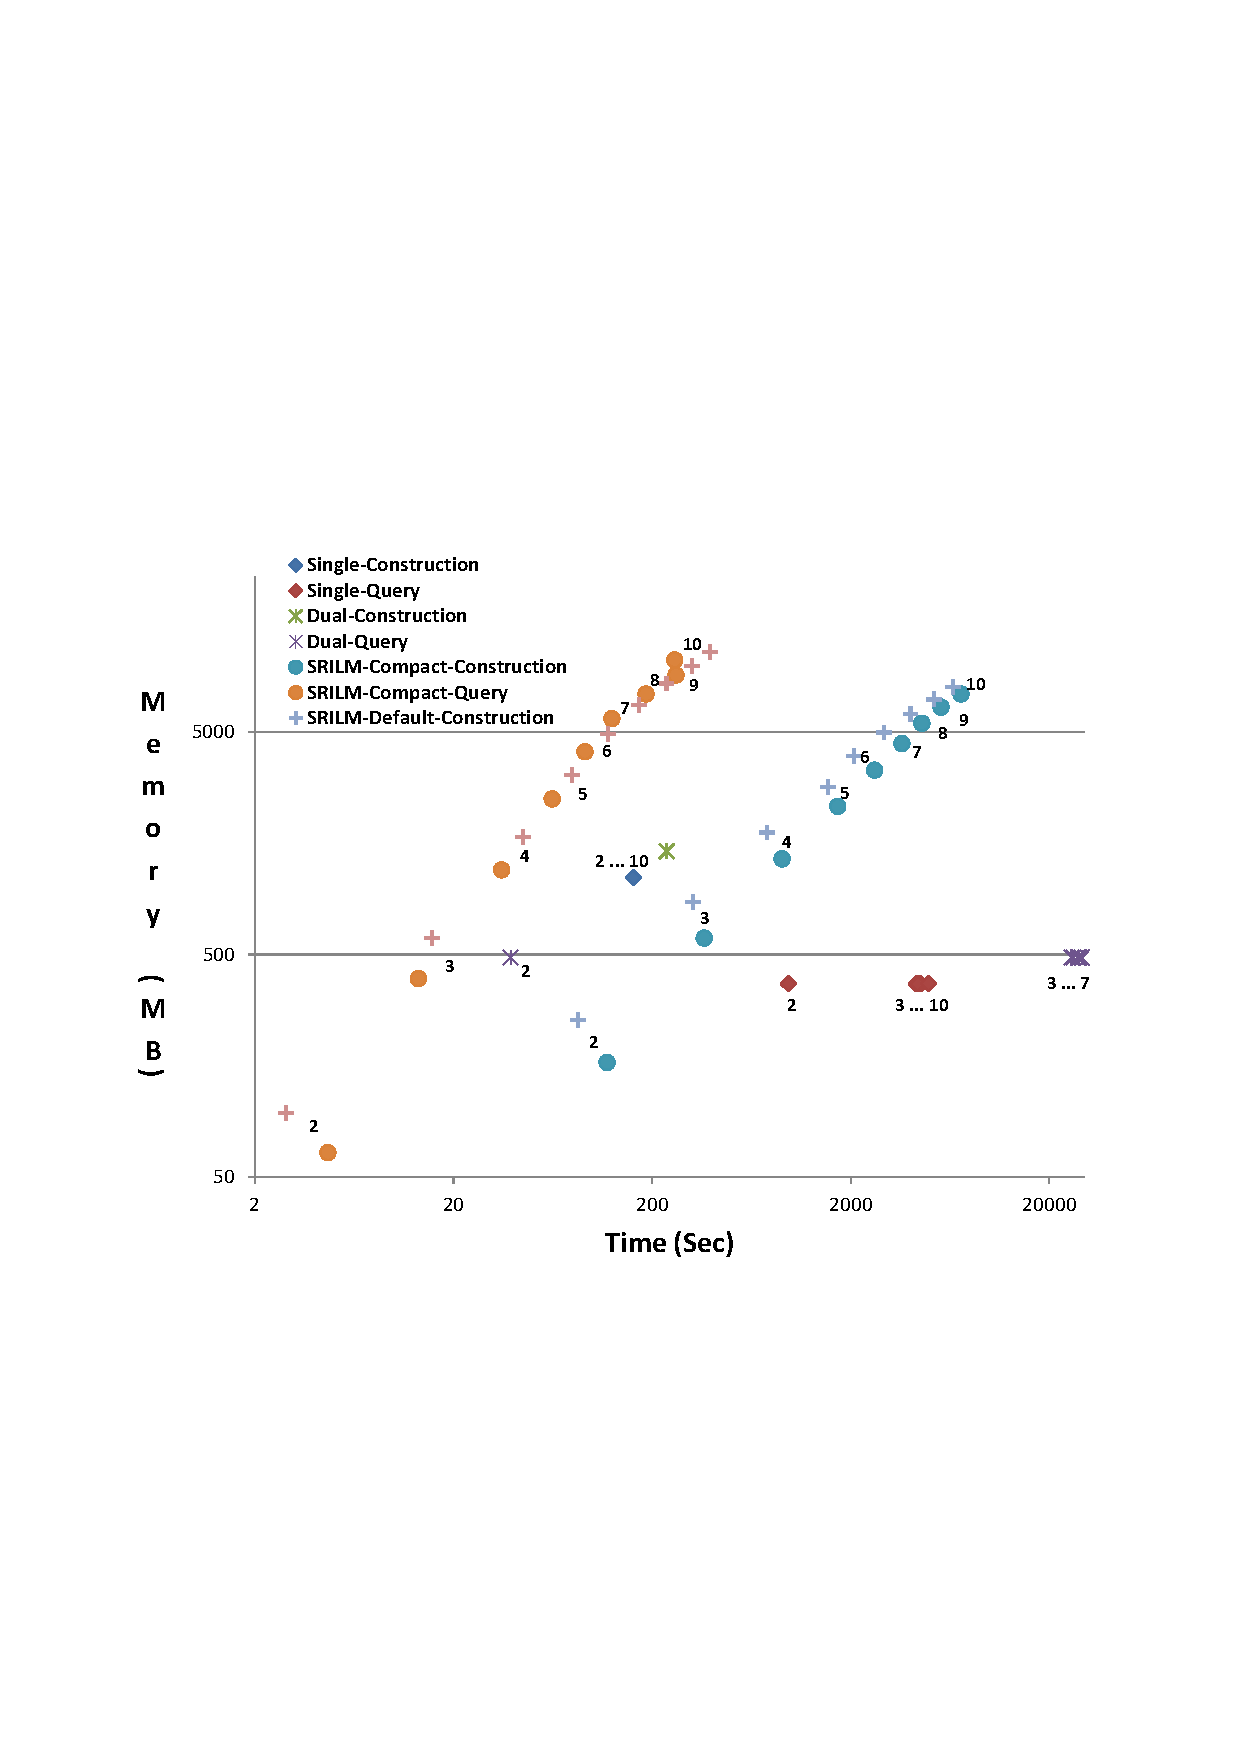
\includegraphics[width=\columnwidth]{figures/Time-Space.pdf}
\caption{On German, showing the size in MB (y axis) and time (x axis) for 4 methods: CST single, CST dual, SRILM, SRILM compact.}
\end{figure}

\missingfigure[figwidth=\columnwidth]{Wikipedia pplx (right axis), and time (left axis) for the single CST on characters vs words as a function of \ngram size.}

\missingfigure[figwidth=\columnwidth]{Wikipedia histogram over \ngram size, perhaps as a figure or table?}

\missingfigure[figwidth=\columnwidth]{Wikipedia plot (stacked bar?) of time spent in each method (n1+ x 3; backward search etc) as a function of n.}


\subsection{Perplexity Evaluation}




%%% Local Variables: 
%%% mode: latex
%%% TeX-master: "cstlm"
%%% End: 
